\vspace{0.5cm}

\begin{enumerate}[1)]
	\item Agregamos el atributo instancia como un entero de la sigiuente forma en el \textit{private}:
		\begin{lstlisting}
private:

   std::string Frase;
   int ID;

   static int Numero;
		\end{lstlisting}
	\item Sea asigna el valor $ID$ igual al atributo Número:
		\begin{figure}[H]
			\centering
			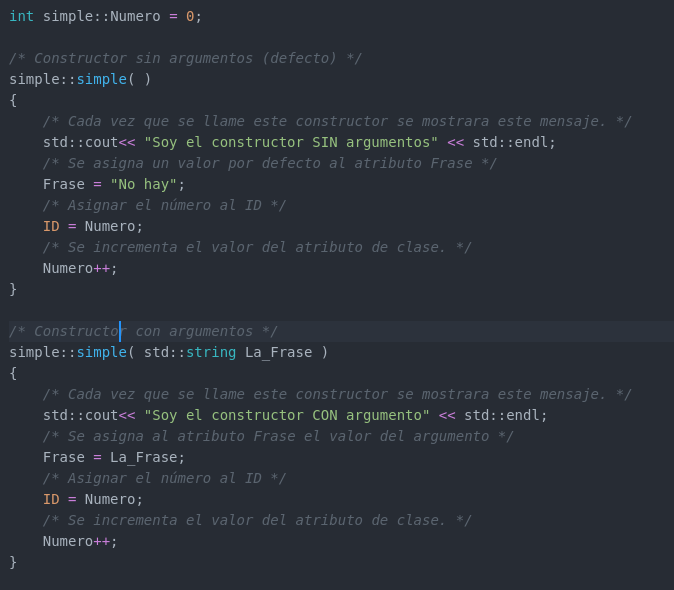
\includegraphics[scale=0.5]{./img/id_numero.png}
		\end{figure}
	\item Se agrega el método
		\begin{lstlisting}
	void Mostrar_ID();
		\end{lstlisting}
		Y se define lo que hace la función
		\begin{lstlisting}
	void simple::Mostrar_ID(){
    	std::cout << "El ID de la instancia es: " << ID << std::endl;
	}
		\end{lstlisting}
	\item Se agrega el nuevo método en el archivo \texttt{class01.cpp} y queda de la siguiente forma
		\begin{figure}[H]
			\centering
			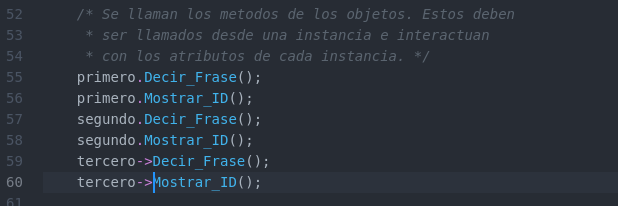
\includegraphics[scale=0.5]{./img/class01.png}
		\end{figure}
	De modo que el output es
		\begin{figure}[H]
			\centering
			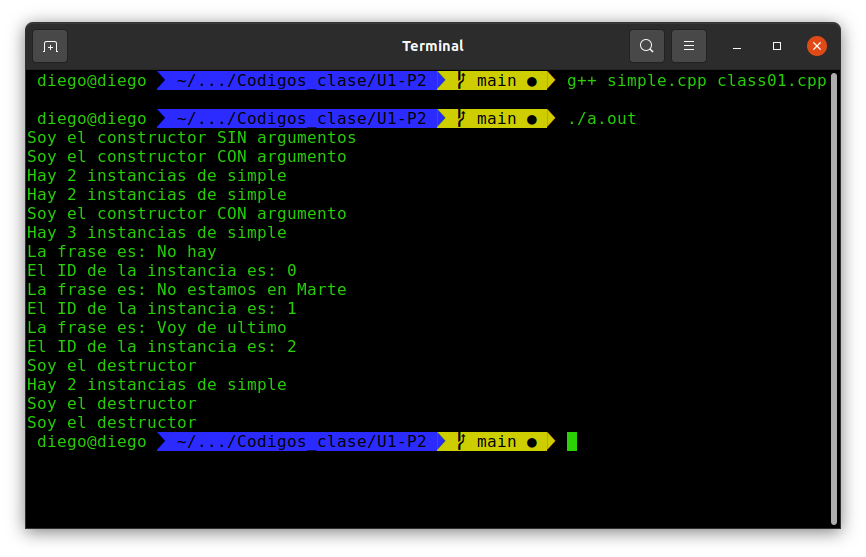
\includegraphics[scale=0.5]{./img/output.png}
		\end{figure}
\end{enumerate}



